\documentclass[1p]{elsarticle_modified}
%\bibliographystyle{elsarticle-num}

%\usepackage[colorlinks]{hyperref}
%\usepackage{abbrmath_seonhwa} %\Abb, \Ascr, \Acal ,\Abf, \Afrak
\usepackage{amsfonts}
\usepackage{amssymb}
\usepackage{amsmath}
\usepackage{amsthm}
\usepackage{scalefnt}
\usepackage{amsbsy}
\usepackage{kotex}
\usepackage{caption}
\usepackage{subfig}
\usepackage{color}
\usepackage{graphicx}
\usepackage{xcolor} %% white, black, red, green, blue, cyan, magenta, yellow
\usepackage{float}
\usepackage{setspace}
\usepackage{hyperref}

\usepackage{tikz}
\usetikzlibrary{arrows}

\usepackage{multirow}
\usepackage{array} % fixed length table
\usepackage{hhline}

%%%%%%%%%%%%%%%%%%%%%
\makeatletter
\renewcommand*\env@matrix[1][\arraystretch]{%
	\edef\arraystretch{#1}%
	\hskip -\arraycolsep
	\let\@ifnextchar\new@ifnextchar
	\array{*\c@MaxMatrixCols c}}
\makeatother %https://tex.stackexchange.com/questions/14071/how-can-i-increase-the-line-spacing-in-a-matrix
%%%%%%%%%%%%%%%

\usepackage[normalem]{ulem}

\newcommand{\msout}[1]{\ifmmode\text{\sout{\ensuremath{#1}}}\else\sout{#1}\fi}
%SOURCE: \msout is \stkout macro in https://tex.stackexchange.com/questions/20609/strikeout-in-math-mode

\newcommand{\cancel}[1]{
	\ifmmode
	{\color{red}\msout{#1}}
	\else
	{\color{red}\sout{#1}}
	\fi
}

\newcommand{\add}[1]{
	{\color{blue}\uwave{#1}}
}

\newcommand{\replace}[2]{
	\ifmmode
	{\color{red}\msout{#1}}{\color{blue}\uwave{#2}}
	\else
	{\color{red}\sout{#1}}{\color{blue}\uwave{#2}}
	\fi
}

\newcommand{\Sol}{\mathcal{S}} %segment
\newcommand{\D}{D} %diagram
\newcommand{\A}{\mathcal{A}} %arc


%%%%%%%%%%%%%%%%%%%%%%%%%%%%%5 test

\def\sl{\operatorname{\textup{SL}}(2,\Cbb)}
\def\psl{\operatorname{\textup{PSL}}(2,\Cbb)}
\def\quan{\mkern 1mu \triangleright \mkern 1mu}

\theoremstyle{definition}
\newtheorem{thm}{Theorem}[section]
\newtheorem{prop}[thm]{Proposition}
\newtheorem{lem}[thm]{Lemma}
\newtheorem{ques}[thm]{Question}
\newtheorem{cor}[thm]{Corollary}
\newtheorem{defn}[thm]{Definition}
\newtheorem{exam}[thm]{Example}
\newtheorem{rmk}[thm]{Remark}
\newtheorem{alg}[thm]{Algorithm}

\newcommand{\I}{\sqrt{-1}}
\begin{document}

%\begin{frontmatter}
%
%\title{Boundary parabolic representations of knots up to 8 crossings}
%
%%% Group authors per affiliation:
%\author{Yunhi Cho} 
%\address{Department of Mathematics, University of Seoul, Seoul, Korea}
%\ead{yhcho@uos.ac.kr}
%
%
%\author{Seonhwa Kim} %\fnref{s_kim}}
%\address{Center for Geometry and Physics, Institute for Basic Science, Pohang, 37673, Korea}
%\ead{ryeona17@ibs.re.kr}
%
%\author{Hyuk Kim}
%\address{Department of Mathematical Sciences, Seoul National University, Seoul 08826, Korea}
%\ead{hyukkim@snu.ac.kr}
%
%\author{Seokbeom Yoon}
%\address{Department of Mathematical Sciences, Seoul National University, Seoul, 08826,  Korea}
%\ead{sbyoon15@snu.ac.kr}
%
%\begin{abstract}
%We find all boundary parabolic representation of knots up to 8 crossings.
%
%\end{abstract}
%\begin{keyword}
%    \MSC[2010] 57M25 
%\end{keyword}
%
%\end{frontmatter}

%\linenumbers
%\tableofcontents
%
\newcommand\colored[1]{\textcolor{white}{\rule[-0.35ex]{0.8em}{1.4ex}}\kern-0.8em\color{red} #1}%
%\newcommand\colored[1]{\textcolor{white}{ #1}\kern-2.17ex	\textcolor{white}{ #1}\kern-1.81ex	\textcolor{white}{ #1}\kern-2.15ex\color{red}#1	}

{\Large $\underline{11a_{133}~(K11a_{133})}$}

\setlength{\tabcolsep}{10pt}
\renewcommand{\arraystretch}{1.6}
\vspace{1cm}\begin{tabular}{m{100pt}>{\centering\arraybackslash}m{274pt}}
\multirow{5}{120pt}{
	\centering
	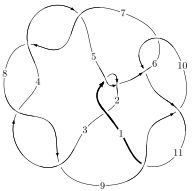
\includegraphics[width=112pt]{../../../GIT/diagram.site/Diagrams/png/382_11a_133.png}\\
\ \ \ A knot diagram\footnotemark}&
\allowdisplaybreaks
\textbf{Linearized knot diagam} \\
\cline{2-2}
 &
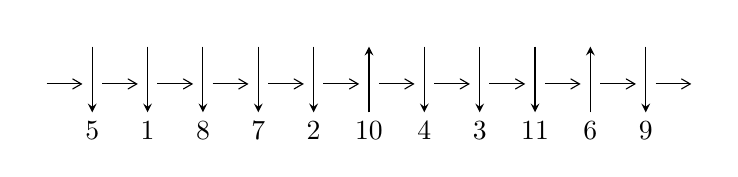
\begin{tikzpicture}[x=20pt, y=17pt]
	% nodes
	\node (C0) at (0, 0) {};
	\node (C1) at (1, 0) {};
	\node (C1U) at (1, +1) {};
	\node (C1D) at (1, -1) {5};

	\node (C2) at (2, 0) {};
	\node (C2U) at (2, +1) {};
	\node (C2D) at (2, -1) {1};

	\node (C3) at (3, 0) {};
	\node (C3U) at (3, +1) {};
	\node (C3D) at (3, -1) {8};

	\node (C4) at (4, 0) {};
	\node (C4U) at (4, +1) {};
	\node (C4D) at (4, -1) {7};

	\node (C5) at (5, 0) {};
	\node (C5U) at (5, +1) {};
	\node (C5D) at (5, -1) {2};

	\node (C6) at (6, 0) {};
	\node (C6U) at (6, +1) {};
	\node (C6D) at (6, -1) {10};

	\node (C7) at (7, 0) {};
	\node (C7U) at (7, +1) {};
	\node (C7D) at (7, -1) {4};

	\node (C8) at (8, 0) {};
	\node (C8U) at (8, +1) {};
	\node (C8D) at (8, -1) {3};

	\node (C9) at (9, 0) {};
	\node (C9U) at (9, +1) {};
	\node (C9D) at (9, -1) {11};

	\node (C10) at (10, 0) {};
	\node (C10U) at (10, +1) {};
	\node (C10D) at (10, -1) {6};

	\node (C11) at (11, 0) {};
	\node (C11U) at (11, +1) {};
	\node (C11D) at (11, -1) {9};
	\node (C12) at (12, 0) {};

	% arrows
	\draw[->,>={angle 60}]
	(C0) edge (C1) (C1) edge (C2) (C2) edge (C3) (C3) edge (C4) (C4) edge (C5) (C5) edge (C6) (C6) edge (C7) (C7) edge (C8) (C8) edge (C9) (C9) edge (C10) (C10) edge (C11) (C11) edge (C12) ;	\draw[->,>=stealth]
	(C1U) edge (C1D) (C2U) edge (C2D) (C3U) edge (C3D) (C4U) edge (C4D) (C5U) edge (C5D) (C6D) edge (C6U) (C7U) edge (C7D) (C8U) edge (C8D) (C9U) edge (C9D) (C10D) edge (C10U) (C11U) edge (C11D) ;
	\end{tikzpicture} \\
\hhline{~~} \\& 
\textbf{Solving Sequence} \\ \cline{2-2} 
 &
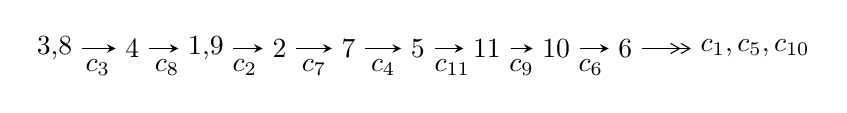
\begin{tikzpicture}[x=25pt, y=7pt]
	% node
	\node (A0) at (-1/8, 0) {3,8};
	\node (A1) at (1, 0) {4};
	\node (A2) at (33/16, 0) {1,9};
	\node (A3) at (25/8, 0) {2};
	\node (A4) at (33/8, 0) {7};
	\node (A5) at (41/8, 0) {5};
	\node (A6) at (49/8, 0) {11};
	\node (A7) at (57/8, 0) {10};
	\node (A8) at (65/8, 0) {6};
	\node (C1) at (1/2, -1) {$c_{3}$};
	\node (C2) at (3/2, -1) {$c_{8}$};
	\node (C3) at (21/8, -1) {$c_{2}$};
	\node (C4) at (29/8, -1) {$c_{7}$};
	\node (C5) at (37/8, -1) {$c_{4}$};
	\node (C6) at (45/8, -1) {$c_{11}$};
	\node (C7) at (53/8, -1) {$c_{9}$};
	\node (C8) at (61/8, -1) {$c_{6}$};
	\node (A9) at (10, 0) {$c_{1},c_{5},c_{10}$};

	% edge
	\draw[->,>=stealth]	
	(A0) edge (A1) (A1) edge (A2) (A2) edge (A3) (A3) edge (A4) (A4) edge (A5) (A5) edge (A6) (A6) edge (A7) (A7) edge (A8) ;
	\draw[->>,>={angle 60}]	
	(A8) edge (A9);
\end{tikzpicture} \\ 

\end{tabular} \\

\footnotetext{
The image of knot diagram is generated by the software ``\textbf{Draw programme}" developed by Andrew Bartholomew(\url{http://www.layer8.co.uk/maths/draw/index.htm\#Running-draw}), where we modified some parts for our purpose(\url{https://github.com/CATsTAILs/LinksPainter}).
}\phantom \\ \newline 
\centering \textbf{Ideals for irreducible components\footnotemark of $X_{\text{par}}$} 
 
\begin{align*}
I^u_{1}&=\langle 
3.79178\times10^{22} u^{44}+3.67398\times10^{22} u^{43}+\cdots+7.16385\times10^{22} b-6.36327\times10^{21},\\
\phantom{I^u_{1}}&\phantom{= \langle  }-9.16718\times10^{20} u^{44}+1.82694\times10^{23} u^{43}+\cdots+2.86554\times10^{23} a-2.62927\times10^{24},\;u^{45}+u^{44}+\cdots-28 u^2-4\rangle \\
I^u_{2}&=\langle 
b+1,\;2 a^2- a u-4 a+u+1,\;u^2+2\rangle \\
\\
I^v_{1}&=\langle 
a,\;b+1,\;v^2+v+1\rangle \\
\end{align*}
\raggedright * 3 irreducible components of $\dim_{\mathbb{C}}=0$, with total 51 representations.\\
\footnotetext{All coefficients of polynomials are rational numbers. But the coefficients are sometimes approximated in decimal forms when there is not enough margin.}
\newpage
\renewcommand{\arraystretch}{1}
\centering \section*{I. $I^u_{1}= \langle 3.79\times10^{22} u^{44}+3.67\times10^{22} u^{43}+\cdots+7.16\times10^{22} b-6.36\times10^{21},\;-9.17\times10^{20} u^{44}+1.83\times10^{23} u^{43}+\cdots+2.87\times10^{23} a-2.63\times10^{24},\;u^{45}+u^{44}+\cdots-28 u^2-4 \rangle$}
\flushleft \textbf{(i) Arc colorings}\\
\begin{tabular}{m{7pt} m{180pt} m{7pt} m{180pt} }
\flushright $a_{3}=$&$\begin{pmatrix}1\\0\end{pmatrix}$ \\
\flushright $a_{8}=$&$\begin{pmatrix}0\\u\end{pmatrix}$ \\
\flushright $a_{4}=$&$\begin{pmatrix}1\\u^2\end{pmatrix}$ \\
\flushright $a_{1}=$&$\begin{pmatrix}0.00319911 u^{44}-0.637556 u^{43}+\cdots-7.59140 u+9.17549\\-0.529294 u^{44}-0.512850 u^{43}+\cdots+4.30006 u+0.0888247\end{pmatrix}$ \\
\flushright $a_{9}=$&$\begin{pmatrix}- u\\u\end{pmatrix}$ \\
\flushright $a_{2}=$&$\begin{pmatrix}0.424417 u^{44}+0.198789 u^{43}+\cdots-8.45475 u+5.64275\\-1.00162 u^{44}-1.22215 u^{43}+\cdots+7.67645 u+1.88551\end{pmatrix}$ \\
\flushright $a_{7}=$&$\begin{pmatrix}u\\u^3+u\end{pmatrix}$ \\
\flushright $a_{5}=$&$\begin{pmatrix}u^2+1\\u^4+2 u^2\end{pmatrix}$ \\
\flushright $a_{11}=$&$\begin{pmatrix}0.432131 u^{44}+0.147580 u^{43}+\cdots-9.69578 u+6.67824\\-0.958226 u^{44}-1.29799 u^{43}+\cdots+6.40444 u+2.58607\end{pmatrix}$ \\
\flushright $a_{10}=$&$\begin{pmatrix}0.729800 u^{44}+0.582734 u^{43}+\cdots-6.09901 u-6.26113\\-0.0344386 u^{44}+0.939991 u^{43}+\cdots+4.74682 u-5.61829\end{pmatrix}$ \\
\flushright $a_{6}=$&$\begin{pmatrix}0.432131 u^{44}+0.147580 u^{43}+\cdots-9.69578 u+6.67824\\0.415034 u^{44}+0.460313 u^{43}+\cdots-4.67591 u-3.72428\end{pmatrix}$\\ \flushright $a_{6}=$&$\begin{pmatrix}0.432131 u^{44}+0.147580 u^{43}+\cdots-9.69578 u+6.67824\\0.415034 u^{44}+0.460313 u^{43}+\cdots-4.67591 u-3.72428\end{pmatrix}$\\&\end{tabular}
\flushleft \textbf{(ii) Obstruction class $= -1$}\\~\\
\flushleft \textbf{(iii) Cusp Shapes $= -\frac{32120453352253218896835}{71638476266902618700479} u^{44}+\frac{51439144552236413356159}{71638476266902618700479} u^{43}+\cdots+\frac{267057572611973423431852}{71638476266902618700479} u-\frac{630536796005845775981388}{71638476266902618700479}$}\\~\\
\newpage\renewcommand{\arraystretch}{1}
\flushleft \textbf{(iv) u-Polynomials at the component}\newline \\
\begin{tabular}{m{50pt}|m{274pt}}
Crossings & \hspace{64pt}u-Polynomials at each crossing \\
\hline $$\begin{aligned}c_{1},c_{5}\end{aligned}$$&$\begin{aligned}
&u^{45}+3 u^{44}+\cdots-10 u+3
\end{aligned}$\\
\hline $$\begin{aligned}c_{2}\end{aligned}$$&$\begin{aligned}
&u^{45}+19 u^{44}+\cdots+58 u+9
\end{aligned}$\\
\hline $$\begin{aligned}c_{3},c_{4},c_{7}\\c_{8}\end{aligned}$$&$\begin{aligned}
&u^{45}- u^{44}+\cdots+28 u^2+4
\end{aligned}$\\
\hline $$\begin{aligned}c_{6},c_{10}\end{aligned}$$&$\begin{aligned}
&u^{45}-2 u^{44}+\cdots+3 u+3
\end{aligned}$\\
\hline $$\begin{aligned}c_{9},c_{11}\end{aligned}$$&$\begin{aligned}
&u^{45}+14 u^{44}+\cdots+21 u-9
\end{aligned}$\\
\hline
\end{tabular}\\~\\
\newpage\renewcommand{\arraystretch}{1}
\flushleft \textbf{(v) Riley Polynomials at the component}\newline \\
\begin{tabular}{m{50pt}|m{274pt}}
Crossings & \hspace{64pt}Riley Polynomials at each crossing \\
\hline $$\begin{aligned}c_{1},c_{5}\end{aligned}$$&$\begin{aligned}
&y^{45}-19 y^{44}+\cdots+58 y-9
\end{aligned}$\\
\hline $$\begin{aligned}c_{2}\end{aligned}$$&$\begin{aligned}
&y^{45}+21 y^{44}+\cdots-1838 y-81
\end{aligned}$\\
\hline $$\begin{aligned}c_{3},c_{4},c_{7}\\c_{8}\end{aligned}$$&$\begin{aligned}
&y^{45}+55 y^{44}+\cdots-224 y-16
\end{aligned}$\\
\hline $$\begin{aligned}c_{6},c_{10}\end{aligned}$$&$\begin{aligned}
&y^{45}+14 y^{44}+\cdots+21 y-9
\end{aligned}$\\
\hline $$\begin{aligned}c_{9},c_{11}\end{aligned}$$&$\begin{aligned}
&y^{45}+38 y^{44}+\cdots+10737 y-81
\end{aligned}$\\
\hline
\end{tabular}\\~\\
\newpage\flushleft \textbf{(vi) Complex Volumes and Cusp Shapes}
$$\begin{array}{c|c|c}  
\text{Solutions to }I^u_{1}& \I (\text{vol} + \sqrt{-1}CS) & \text{Cusp shape}\\
 \hline 
\begin{aligned}
u &= -0.595154 + 0.799976 I \\
a &= -0.809139 - 0.923508 I \\
b &= -0.66293 + 1.48925 I\end{aligned}
 & \phantom{-}3.82469 + 9.97213 I & -4.07711 - 8.66746 I \\ \hline\begin{aligned}
u &= -0.595154 - 0.799976 I \\
a &= -0.809139 + 0.923508 I \\
b &= -0.66293 - 1.48925 I\end{aligned}
 & \phantom{-}3.82469 - 9.97213 I & -4.07711 + 8.66746 I \\ \hline\begin{aligned}
u &= \phantom{-}0.542227 + 0.847104 I \\
a &= -0.624429 + 0.873722 I \\
b &= -0.49486 - 1.41856 I\end{aligned}
 & \phantom{-}4.60680 - 4.00969 I & -2.37481 + 3.81201 I \\ \hline\begin{aligned}
u &= \phantom{-}0.542227 - 0.847104 I \\
a &= -0.624429 - 0.873722 I \\
b &= -0.49486 + 1.41856 I\end{aligned}
 & \phantom{-}4.60680 + 4.00969 I & -2.37481 - 3.81201 I \\ \hline\begin{aligned}
u &= \phantom{-}0.449130 + 0.919217 I \\
a &= \phantom{-}0.997189 - 0.562134 I \\
b &= \phantom{-}0.360475 + 0.942383 I\end{aligned}
 & \phantom{-}5.31668 - 4.26099 I & -1.24439 + 3.98671 I \\ \hline\begin{aligned}
u &= \phantom{-}0.449130 - 0.919217 I \\
a &= \phantom{-}0.997189 + 0.562134 I \\
b &= \phantom{-}0.360475 - 0.942383 I\end{aligned}
 & \phantom{-}5.31668 + 4.26099 I & -1.24439 - 3.98671 I \\ \hline\begin{aligned}
u &= -0.372392 + 1.006660 I \\
a &= \phantom{-}0.981655 + 0.526640 I \\
b &= \phantom{-}0.139519 - 1.024240 I\end{aligned}
 & \phantom{-}5.57757 - 1.59310 I & -0.70414 + 1.88658 I \\ \hline\begin{aligned}
u &= -0.372392 - 1.006660 I \\
a &= \phantom{-}0.981655 - 0.526640 I \\
b &= \phantom{-}0.139519 + 1.024240 I\end{aligned}
 & \phantom{-}5.57757 + 1.59310 I & -0.70414 - 1.88658 I \\ \hline\begin{aligned}
u &= \phantom{-}0.203852 + 0.752739 I \\
a &= \phantom{-}0.411257 + 1.253590 I \\
b &= -0.370857 - 0.767483 I\end{aligned}
 & \phantom{-}1.25627 - 2.00304 I & -0.90089 + 4.84629 I \\ \hline\begin{aligned}
u &= \phantom{-}0.203852 - 0.752739 I \\
a &= \phantom{-}0.411257 - 1.253590 I \\
b &= -0.370857 + 0.767483 I\end{aligned}
 & \phantom{-}1.25627 + 2.00304 I & -0.90089 - 4.84629 I\\
 \hline 
 \end{array}$$\newpage$$\begin{array}{c|c|c}  
\text{Solutions to }I^u_{1}& \I (\text{vol} + \sqrt{-1}CS) & \text{Cusp shape}\\
 \hline 
\begin{aligned}
u &= -0.756562 + 0.151657 I \\
a &= \phantom{-}0.353008 - 0.645751 I \\
b &= -0.400769 - 1.209730 I\end{aligned}
 & \phantom{-}1.87890 - 5.45220 I & -5.89309 + 4.91113 I \\ \hline\begin{aligned}
u &= -0.756562 - 0.151657 I \\
a &= \phantom{-}0.353008 + 0.645751 I \\
b &= -0.400769 + 1.209730 I\end{aligned}
 & \phantom{-}1.87890 + 5.45220 I & -5.89309 - 4.91113 I \\ \hline\begin{aligned}
u &= -0.411509 + 0.629213 I \\
a &= -0.48287 - 1.77369 I \\
b &= -0.759126 + 0.924061 I\end{aligned}
 & -2.33846 + 4.64978 I & -9.14624 - 8.10002 I \\ \hline\begin{aligned}
u &= -0.411509 - 0.629213 I \\
a &= -0.48287 + 1.77369 I \\
b &= -0.759126 - 0.924061 I\end{aligned}
 & -2.33846 - 4.64978 I & -9.14624 + 8.10002 I \\ \hline\begin{aligned}
u &= \phantom{-}0.739174 + 0.066659 I \\
a &= \phantom{-}0.432504 + 0.605344 I \\
b &= -0.183861 + 1.069320 I\end{aligned}
 & \phantom{-}2.24775 - 0.28638 I & -4.98856 + 0.17511 I \\ \hline\begin{aligned}
u &= \phantom{-}0.739174 - 0.066659 I \\
a &= \phantom{-}0.432504 - 0.605344 I \\
b &= -0.183861 - 1.069320 I\end{aligned}
 & \phantom{-}2.24775 + 0.28638 I & -4.98856 - 0.17511 I \\ \hline\begin{aligned}
u &= \phantom{-}0.038629 + 1.346620 I \\
a &= \phantom{-}0.753383 - 0.039929 I \\
b &= -0.056494 - 0.156524 I\end{aligned}
 & \phantom{-}4.91236 - 2.29181 I & \phantom{-0.000000 } 0 \\ \hline\begin{aligned}
u &= \phantom{-}0.038629 - 1.346620 I \\
a &= \phantom{-}0.753383 + 0.039929 I \\
b &= -0.056494 + 0.156524 I\end{aligned}
 & \phantom{-}4.91236 + 2.29181 I & \phantom{-0.000000 } 0 \\ \hline\begin{aligned}
u &= -0.101635 + 0.590584 I \\
a &= -0.429318 - 0.140632 I \\
b &= -1.47830 - 0.11239 I\end{aligned}
 & -0.78716 + 2.48122 I & -3.04347 - 4.76589 I \\ \hline\begin{aligned}
u &= -0.101635 - 0.590584 I \\
a &= -0.429318 + 0.140632 I \\
b &= -1.47830 + 0.11239 I\end{aligned}
 & -0.78716 - 2.48122 I & -3.04347 + 4.76589 I\\
 \hline 
 \end{array}$$\newpage$$\begin{array}{c|c|c}  
\text{Solutions to }I^u_{1}& \I (\text{vol} + \sqrt{-1}CS) & \text{Cusp shape}\\
 \hline 
\begin{aligned}
u &= -0.479511 + 0.303305 I \\
a &= \phantom{-}0.065872 - 0.427985 I \\
b &= -0.987241 - 0.640209 I\end{aligned}
 & -3.30905 - 1.49655 I & -13.54204 - 0.04800 I \\ \hline\begin{aligned}
u &= -0.479511 - 0.303305 I \\
a &= \phantom{-}0.065872 + 0.427985 I \\
b &= -0.987241 + 0.640209 I\end{aligned}
 & -3.30905 + 1.49655 I & -13.54204 + 0.04800 I \\ \hline\begin{aligned}
u &= -0.08818 + 1.43765 I \\
a &= \phantom{-}1.047830 + 0.106631 I \\
b &= -1.143340 - 0.464536 I\end{aligned}
 & \phantom{-}2.28059 + 0.33440 I & \phantom{-0.000000 } 0 \\ \hline\begin{aligned}
u &= -0.08818 - 1.43765 I \\
a &= \phantom{-}1.047830 - 0.106631 I \\
b &= -1.143340 + 0.464536 I\end{aligned}
 & \phantom{-}2.28059 - 0.33440 I & \phantom{-0.000000 } 0 \\ \hline\begin{aligned}
u &= -0.117374 + 0.488254 I \\
a &= \phantom{-}1.95300 - 2.18078 I \\
b &= -0.572552 + 0.344300 I\end{aligned}
 & -1.01308 - 1.54097 I & -3.12750 - 1.49729 I \\ \hline\begin{aligned}
u &= -0.117374 - 0.488254 I \\
a &= \phantom{-}1.95300 + 2.18078 I \\
b &= -0.572552 - 0.344300 I\end{aligned}
 & -1.01308 + 1.54097 I & -3.12750 + 1.49729 I \\ \hline\begin{aligned}
u &= \phantom{-}0.320837 + 0.380710 I \\
a &= \phantom{-}1.001570 - 0.386206 I \\
b &= \phantom{-}0.159215 + 0.077837 I\end{aligned}
 & -0.430811 - 1.192020 I & -5.27697 + 5.64355 I \\ \hline\begin{aligned}
u &= \phantom{-}0.320837 - 0.380710 I \\
a &= \phantom{-}1.001570 + 0.386206 I \\
b &= \phantom{-}0.159215 - 0.077837 I\end{aligned}
 & -0.430811 + 1.192020 I & -5.27697 - 5.64355 I \\ \hline\begin{aligned}
u &= -0.00060 + 1.58402 I \\
a &= \phantom{-}0.58858 - 1.61169 I \\
b &= -0.042622 + 0.922347 I\end{aligned}
 & \phantom{-}6.21731 - 1.33164 I & \phantom{-0.000000 } 0 \\ \hline\begin{aligned}
u &= -0.00060 - 1.58402 I \\
a &= \phantom{-}0.58858 + 1.61169 I \\
b &= -0.042622 - 0.922347 I\end{aligned}
 & \phantom{-}6.21731 + 1.33164 I & \phantom{-0.000000 } 0\\
 \hline 
 \end{array}$$\newpage$$\begin{array}{c|c|c}  
\text{Solutions to }I^u_{1}& \I (\text{vol} + \sqrt{-1}CS) & \text{Cusp shape}\\
 \hline 
\begin{aligned}
u &= -0.10202 + 1.59722 I \\
a &= \phantom{-}0.16838 - 2.06884 I \\
b &= -0.568246 + 1.291280 I\end{aligned}
 & \phantom{-}5.28483 + 6.46491 I & \phantom{-0.000000 } 0 \\ \hline\begin{aligned}
u &= -0.10202 - 1.59722 I \\
a &= \phantom{-}0.16838 + 2.06884 I \\
b &= -0.568246 - 1.291280 I\end{aligned}
 & \phantom{-}5.28483 - 6.46491 I & \phantom{-0.000000 } 0 \\ \hline\begin{aligned}
u &= \phantom{-}0.393229\phantom{ +0.000000I} \\
a &= \phantom{-}0.318039\phantom{ +0.000000I} \\
b &= -0.551275\phantom{ +0.000000I}\end{aligned}
 & -0.995192\phantom{ +0.000000I} & -10.6150\phantom{ +0.000000I} \\ \hline\begin{aligned}
u &= -0.02225 + 1.60699 I \\
a &= \phantom{-}1.205480 + 0.019298 I \\
b &= -2.04934 - 0.12580 I\end{aligned}
 & \phantom{-}6.93943 + 2.89736 I & \phantom{-0.000000 } 0 \\ \hline\begin{aligned}
u &= -0.02225 - 1.60699 I \\
a &= \phantom{-}1.205480 - 0.019298 I \\
b &= -2.04934 + 0.12580 I\end{aligned}
 & \phantom{-}6.93943 - 2.89736 I & \phantom{-0.000000 } 0 \\ \hline\begin{aligned}
u &= \phantom{-}0.04744 + 1.63431 I \\
a &= \phantom{-}0.24569 + 1.76495 I \\
b &= -0.161409 - 1.339170 I\end{aligned}
 & \phantom{-}9.56075 - 2.89885 I & \phantom{-0.000000 } 0 \\ \hline\begin{aligned}
u &= \phantom{-}0.04744 - 1.63431 I \\
a &= \phantom{-}0.24569 - 1.76495 I \\
b &= -0.161409 + 1.339170 I\end{aligned}
 & \phantom{-}9.56075 + 2.89885 I & \phantom{-0.000000 } 0 \\ \hline\begin{aligned}
u &= -0.17946 + 1.64793 I \\
a &= -0.15251 - 1.95899 I \\
b &= -0.85684 + 1.76671 I\end{aligned}
 & \phantom{-}12.1487 + 12.9478 I & \phantom{-0.000000 } 0 \\ \hline\begin{aligned}
u &= -0.17946 - 1.64793 I \\
a &= -0.15251 + 1.95899 I \\
b &= -0.85684 - 1.76671 I\end{aligned}
 & \phantom{-}12.1487 - 12.9478 I & \phantom{-0.000000 } 0 \\ \hline\begin{aligned}
u &= \phantom{-}0.15594 + 1.66197 I \\
a &= -0.10012 + 1.91348 I \\
b &= -0.69213 - 1.78816 I\end{aligned}
 & \phantom{-}13.2084 - 6.7061 I & \phantom{-0.000000 } 0\\
 \hline 
 \end{array}$$\newpage$$\begin{array}{c|c|c}  
\text{Solutions to }I^u_{1}& \I (\text{vol} + \sqrt{-1}CS) & \text{Cusp shape}\\
 \hline 
\begin{aligned}
u &= \phantom{-}0.15594 - 1.66197 I \\
a &= -0.10012 - 1.91348 I \\
b &= -0.69213 + 1.78816 I\end{aligned}
 & \phantom{-}13.2084 + 6.7061 I & \phantom{-0.000000 } 0 \\ \hline\begin{aligned}
u &= \phantom{-}0.11988 + 1.67520 I \\
a &= \phantom{-}0.116060 - 1.188540 I \\
b &= \phantom{-}0.864414 + 1.057190 I\end{aligned}
 & \phantom{-}14.2846 - 6.4583 I & \phantom{-0.000000 } 0 \\ \hline\begin{aligned}
u &= \phantom{-}0.11988 - 1.67520 I \\
a &= \phantom{-}0.116060 + 1.188540 I \\
b &= \phantom{-}0.864414 - 1.057190 I\end{aligned}
 & \phantom{-}14.2846 + 6.4583 I & \phantom{-0.000000 } 0 \\ \hline\begin{aligned}
u &= -0.08709 + 1.68689 I \\
a &= \phantom{-}0.117912 + 1.285170 I \\
b &= \phantom{-}0.73293 - 1.22370 I\end{aligned}
 & \phantom{-}14.9288 + 0.1276 I & \phantom{-0.000000 } 0 \\ \hline\begin{aligned}
u &= -0.08709 - 1.68689 I \\
a &= \phantom{-}0.117912 - 1.285170 I \\
b &= \phantom{-}0.73293 + 1.22370 I\end{aligned}
 & \phantom{-}14.9288 - 0.1276 I & \phantom{-0.000000 } 0\\
 \hline 
 \end{array}$$\newpage\newpage\renewcommand{\arraystretch}{1}
\centering \section*{II. $I^u_{2}= \langle b+1,\;2 a^2- a u-4 a+u+1,\;u^2+2 \rangle$}
\flushleft \textbf{(i) Arc colorings}\\
\begin{tabular}{m{7pt} m{180pt} m{7pt} m{180pt} }
\flushright $a_{3}=$&$\begin{pmatrix}1\\0\end{pmatrix}$ \\
\flushright $a_{8}=$&$\begin{pmatrix}0\\u\end{pmatrix}$ \\
\flushright $a_{4}=$&$\begin{pmatrix}1\\-2\end{pmatrix}$ \\
\flushright $a_{1}=$&$\begin{pmatrix}a\\-1\end{pmatrix}$ \\
\flushright $a_{9}=$&$\begin{pmatrix}- u\\u\end{pmatrix}$ \\
\flushright $a_{2}=$&$\begin{pmatrix}a+1\\-1\end{pmatrix}$ \\
\flushright $a_{7}=$&$\begin{pmatrix}u\\- u\end{pmatrix}$ \\
\flushright $a_{5}=$&$\begin{pmatrix}-1\\0\end{pmatrix}$ \\
\flushright $a_{11}=$&$\begin{pmatrix}- a+2\\2 a-3\end{pmatrix}$ \\
\flushright $a_{10}=$&$\begin{pmatrix}- a u- a+\frac{1}{2} u+1\\a u+2 a- u-2\end{pmatrix}$ \\
\flushright $a_{6}=$&$\begin{pmatrix}a\\-1\end{pmatrix}$\\ \flushright $a_{6}=$&$\begin{pmatrix}a\\-1\end{pmatrix}$\\&\end{tabular}
\flushleft \textbf{(ii) Obstruction class $= 1$}\\~\\
\flushleft \textbf{(iii) Cusp Shapes $= -4 a u+4 u-8$}\\~\\
\newpage\renewcommand{\arraystretch}{1}
\flushleft \textbf{(iv) u-Polynomials at the component}\newline \\
\begin{tabular}{m{50pt}|m{274pt}}
Crossings & \hspace{64pt}u-Polynomials at each crossing \\
\hline $$\begin{aligned}c_{1},c_{2}\end{aligned}$$&$\begin{aligned}
&(u+1)^4
\end{aligned}$\\
\hline $$\begin{aligned}c_{3},c_{4},c_{7}\\c_{8}\end{aligned}$$&$\begin{aligned}
&(u^2+2)^2
\end{aligned}$\\
\hline $$\begin{aligned}c_{5}\end{aligned}$$&$\begin{aligned}
&(u-1)^4
\end{aligned}$\\
\hline $$\begin{aligned}c_{6},c_{9}\end{aligned}$$&$\begin{aligned}
&(u^2- u+1)^2
\end{aligned}$\\
\hline $$\begin{aligned}c_{10},c_{11}\end{aligned}$$&$\begin{aligned}
&(u^2+u+1)^2
\end{aligned}$\\
\hline
\end{tabular}\\~\\
\newpage\renewcommand{\arraystretch}{1}
\flushleft \textbf{(v) Riley Polynomials at the component}\newline \\
\begin{tabular}{m{50pt}|m{274pt}}
Crossings & \hspace{64pt}Riley Polynomials at each crossing \\
\hline $$\begin{aligned}c_{1},c_{2},c_{5}\end{aligned}$$&$\begin{aligned}
&(y-1)^4
\end{aligned}$\\
\hline $$\begin{aligned}c_{3},c_{4},c_{7}\\c_{8}\end{aligned}$$&$\begin{aligned}
&(y+2)^4
\end{aligned}$\\
\hline $$\begin{aligned}c_{6},c_{9},c_{10}\\c_{11}\end{aligned}$$&$\begin{aligned}
&(y^2+y+1)^2
\end{aligned}$\\
\hline
\end{tabular}\\~\\
\newpage\flushleft \textbf{(vi) Complex Volumes and Cusp Shapes}
$$\begin{array}{c|c|c}  
\text{Solutions to }I^u_{2}& \I (\text{vol} + \sqrt{-1}CS) & \text{Cusp shape}\\
 \hline 
\begin{aligned}
u &= \phantom{-0.000000 -}1.414210 I \\
a &= \phantom{-}0.387628 + 0.353553 I \\
b &= -1.00000\phantom{ +0.000000I}\end{aligned}
 & \phantom{-}3.28987 - 2.02988 I & -6.00000 + 3.46410 I \\ \hline\begin{aligned}
u &= \phantom{-0.000000 -}1.414210 I \\
a &= \phantom{-}1.61237 + 0.35355 I \\
b &= -1.00000\phantom{ +0.000000I}\end{aligned}
 & \phantom{-}3.28987 + 2.02988 I & -6.00000 - 3.46410 I \\ \hline\begin{aligned}
u &= \phantom{-0.000000 } -1.414210 I \\
a &= \phantom{-}0.387628 - 0.353553 I \\
b &= -1.00000\phantom{ +0.000000I}\end{aligned}
 & \phantom{-}3.28987 + 2.02988 I & -6.00000 - 3.46410 I \\ \hline\begin{aligned}
u &= \phantom{-0.000000 } -1.414210 I \\
a &= \phantom{-}1.61237 - 0.35355 I \\
b &= -1.00000\phantom{ +0.000000I}\end{aligned}
 & \phantom{-}3.28987 - 2.02988 I & -6.00000 + 3.46410 I\\
 \hline 
 \end{array}$$\newpage\newpage\renewcommand{\arraystretch}{1}
\centering \section*{III. $I^v_{1}= \langle a,\;b+1,\;v^2+v+1 \rangle$}
\flushleft \textbf{(i) Arc colorings}\\
\begin{tabular}{m{7pt} m{180pt} m{7pt} m{180pt} }
\flushright $a_{3}=$&$\begin{pmatrix}1\\0\end{pmatrix}$ \\
\flushright $a_{8}=$&$\begin{pmatrix}v\\0\end{pmatrix}$ \\
\flushright $a_{4}=$&$\begin{pmatrix}1\\0\end{pmatrix}$ \\
\flushright $a_{1}=$&$\begin{pmatrix}0\\-1\end{pmatrix}$ \\
\flushright $a_{9}=$&$\begin{pmatrix}v\\0\end{pmatrix}$ \\
\flushright $a_{2}=$&$\begin{pmatrix}1\\-1\end{pmatrix}$ \\
\flushright $a_{7}=$&$\begin{pmatrix}v\\0\end{pmatrix}$ \\
\flushright $a_{5}=$&$\begin{pmatrix}1\\0\end{pmatrix}$ \\
\flushright $a_{11}=$&$\begin{pmatrix}v+1\\-1\end{pmatrix}$ \\
\flushright $a_{10}=$&$\begin{pmatrix}v+1\\v\end{pmatrix}$ \\
\flushright $a_{6}=$&$\begin{pmatrix}0\\1\end{pmatrix}$\\ \flushright $a_{6}=$&$\begin{pmatrix}0\\1\end{pmatrix}$\\&\end{tabular}
\flushleft \textbf{(ii) Obstruction class $= 1$}\\~\\
\flushleft \textbf{(iii) Cusp Shapes $= -4 v-14$}\\~\\
\newpage\renewcommand{\arraystretch}{1}
\flushleft \textbf{(iv) u-Polynomials at the component}\newline \\
\begin{tabular}{m{50pt}|m{274pt}}
Crossings & \hspace{64pt}u-Polynomials at each crossing \\
\hline $$\begin{aligned}c_{1}\end{aligned}$$&$\begin{aligned}
&(u-1)^2
\end{aligned}$\\
\hline $$\begin{aligned}c_{2},c_{5}\end{aligned}$$&$\begin{aligned}
&(u+1)^2
\end{aligned}$\\
\hline $$\begin{aligned}c_{3},c_{4},c_{7}\\c_{8}\end{aligned}$$&$\begin{aligned}
&u^2
\end{aligned}$\\
\hline $$\begin{aligned}c_{6},c_{11}\end{aligned}$$&$\begin{aligned}
&u^2+u+1
\end{aligned}$\\
\hline $$\begin{aligned}c_{9},c_{10}\end{aligned}$$&$\begin{aligned}
&u^2- u+1
\end{aligned}$\\
\hline
\end{tabular}\\~\\
\newpage\renewcommand{\arraystretch}{1}
\flushleft \textbf{(v) Riley Polynomials at the component}\newline \\
\begin{tabular}{m{50pt}|m{274pt}}
Crossings & \hspace{64pt}Riley Polynomials at each crossing \\
\hline $$\begin{aligned}c_{1},c_{2},c_{5}\end{aligned}$$&$\begin{aligned}
&(y-1)^2
\end{aligned}$\\
\hline $$\begin{aligned}c_{3},c_{4},c_{7}\\c_{8}\end{aligned}$$&$\begin{aligned}
&y^2
\end{aligned}$\\
\hline $$\begin{aligned}c_{6},c_{9},c_{10}\\c_{11}\end{aligned}$$&$\begin{aligned}
&y^2+y+1
\end{aligned}$\\
\hline
\end{tabular}\\~\\
\newpage\flushleft \textbf{(vi) Complex Volumes and Cusp Shapes}
$$\begin{array}{c|c|c}  
\text{Solutions to }I^v_{1}& \I (\text{vol} + \sqrt{-1}CS) & \text{Cusp shape}\\
 \hline 
\begin{aligned}
v &= -0.500000 + 0.866025 I \\
a &= \phantom{-0.000000 } 0 \\
b &= -1.00000\phantom{ +0.000000I}\end{aligned}
 & -1.64493 + 2.02988 I & -12.00000 - 3.46410 I \\ \hline\begin{aligned}
v &= -0.500000 - 0.866025 I \\
a &= \phantom{-0.000000 } 0 \\
b &= -1.00000\phantom{ +0.000000I}\end{aligned}
 & -1.64493 - 2.02988 I & -12.00000 + 3.46410 I\\
 \hline 
 \end{array}$$\newpage
\newpage\renewcommand{\arraystretch}{1}
\centering \section*{ IV. u-Polynomials}
\begin{tabular}{m{50pt}|m{274pt}}
Crossings & \hspace{64pt}u-Polynomials at each crossing \\
\hline $$\begin{aligned}c_{1}\end{aligned}$$&$\begin{aligned}
&((u-1)^2)(u+1)^4(u^{45}+3 u^{44}+\cdots-10 u+3)
\end{aligned}$\\
\hline $$\begin{aligned}c_{2}\end{aligned}$$&$\begin{aligned}
&((u+1)^6)(u^{45}+19 u^{44}+\cdots+58 u+9)
\end{aligned}$\\
\hline $$\begin{aligned}c_{3},c_{4},c_{7}\\c_{8}\end{aligned}$$&$\begin{aligned}
&u^2(u^2+2)^2(u^{45}- u^{44}+\cdots+28 u^2+4)
\end{aligned}$\\
\hline $$\begin{aligned}c_{5}\end{aligned}$$&$\begin{aligned}
&((u-1)^4)(u+1)^2(u^{45}+3 u^{44}+\cdots-10 u+3)
\end{aligned}$\\
\hline $$\begin{aligned}c_{6}\end{aligned}$$&$\begin{aligned}
&((u^2- u+1)^2)(u^2+u+1)(u^{45}-2 u^{44}+\cdots+3 u+3)
\end{aligned}$\\
\hline $$\begin{aligned}c_{9}\end{aligned}$$&$\begin{aligned}
&((u^2- u+1)^3)(u^{45}+14 u^{44}+\cdots+21 u-9)
\end{aligned}$\\
\hline $$\begin{aligned}c_{10}\end{aligned}$$&$\begin{aligned}
&(u^2- u+1)(u^2+u+1)^2(u^{45}-2 u^{44}+\cdots+3 u+3)
\end{aligned}$\\
\hline $$\begin{aligned}c_{11}\end{aligned}$$&$\begin{aligned}
&((u^2+u+1)^3)(u^{45}+14 u^{44}+\cdots+21 u-9)
\end{aligned}$\\
\hline
\end{tabular}\newpage\renewcommand{\arraystretch}{1}
\centering \section*{ V. Riley Polynomials}
\begin{tabular}{m{50pt}|m{274pt}}
Crossings & \hspace{64pt}Riley Polynomials at each crossing \\
\hline $$\begin{aligned}c_{1},c_{5}\end{aligned}$$&$\begin{aligned}
&((y-1)^6)(y^{45}-19 y^{44}+\cdots+58 y-9)
\end{aligned}$\\
\hline $$\begin{aligned}c_{2}\end{aligned}$$&$\begin{aligned}
&((y-1)^6)(y^{45}+21 y^{44}+\cdots-1838 y-81)
\end{aligned}$\\
\hline $$\begin{aligned}c_{3},c_{4},c_{7}\\c_{8}\end{aligned}$$&$\begin{aligned}
&y^2(y+2)^4(y^{45}+55 y^{44}+\cdots-224 y-16)
\end{aligned}$\\
\hline $$\begin{aligned}c_{6},c_{10}\end{aligned}$$&$\begin{aligned}
&((y^2+y+1)^3)(y^{45}+14 y^{44}+\cdots+21 y-9)
\end{aligned}$\\
\hline $$\begin{aligned}c_{9},c_{11}\end{aligned}$$&$\begin{aligned}
&((y^2+y+1)^3)(y^{45}+38 y^{44}+\cdots+10737 y-81)
\end{aligned}$\\
\hline
\end{tabular}
\vskip 2pc
\end{document}